\documentclass{article}
\usepackage{geometry}
\usepackage{longtable}
\usepackage{amsmath}
\usepackage{booktabs}
\usepackage{xcolor}
\usepackage{hyperref}
\usepackage{graphicx} % Required for including images
\geometry{margin=1in}

\title{Summary about dissertation of Zhang (2008) and Vercruysse (2022)Thesis work}

\begin{document}
\maketitle

\begin{center}
    {\Large Abstract}
\end{center}

    In Part 1 and 2 of this document, i summarized the work of Zhang (2008) and Vercruysse et al. (2017) by listing the data, methods and results presented in their work.
    It can be skipped if the summary is not of interest.

    In part 3, i did some coding with simualted data to see how can i quickly reproduce similar results and how could i extend the work.
    These ideas are tentative and not fully developed yet, but i think it is a good start and worth to be included in the report.

The major exploration i did can be concentrated into the figure below, which shows the geographic/spatial exploration(a), 
breakpoint quantile regression(b, c) and PCA by SVD(d).

The code and supportive files can be found in this \textbf{GitHub repository}: \href{https://github.com/Gufeng-2002/Reading_Notes/tree/main}{\textit{src\_test(source of code)}.}

\begin{figure}[!h]
    \centering
    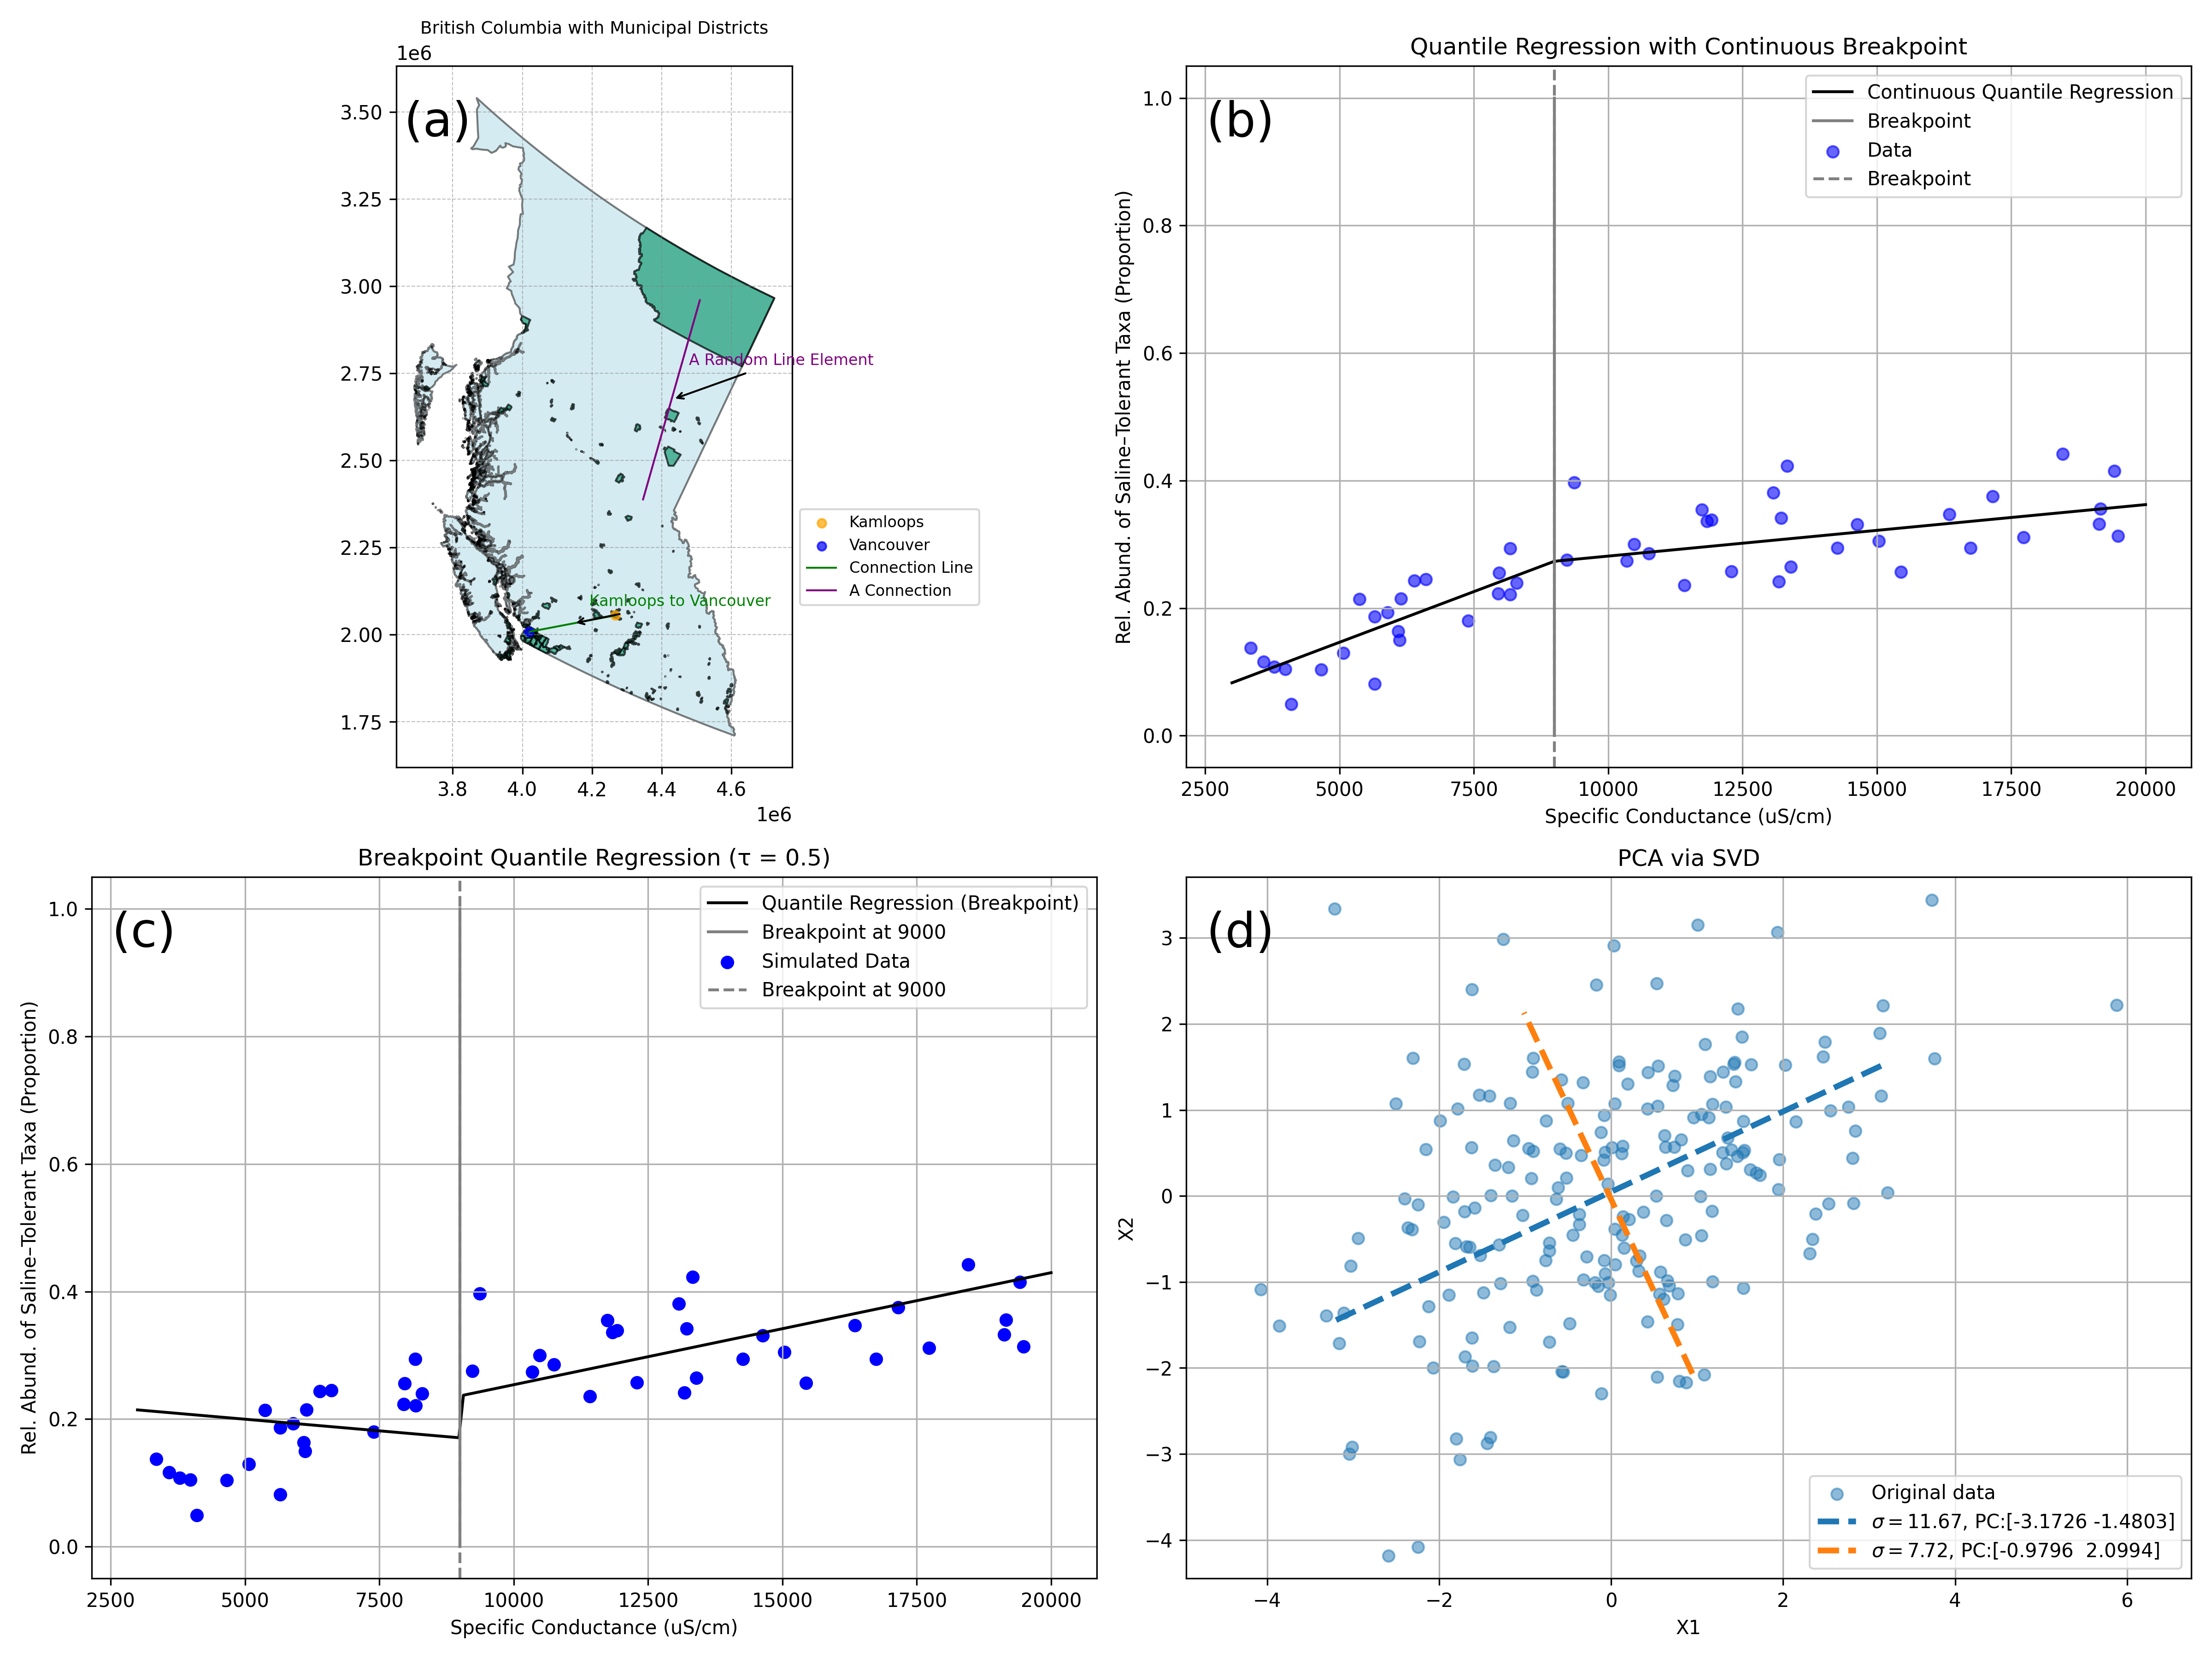
\includegraphics[width=0.9\textwidth]{../src_test/results/combined_plot.png}
    % \caption{\textit{Summary of the major exploration i did}}
    % \label{fig:summary}
\end{figure}


\newpage
\begin{center}
    \tableofcontents
\end{center}


\newpage
\section{Zhang's work (2008)}
The following notes summarize the work of Zhang (2008) on sediment contaminants and their effects on benthic communities in the Great Lakes region. 
The study focuses on the Detroit River and Lake St. Clair, examining the relationship between sediment contamination and zoobenthic community structure.

\subsection{Data sources (Chapter 2)}
\subsubsection*{1. Chemical Variables (Sediment Contaminants)}
\subsubsection*{Grouped by Principal Components (PCA)}
\begin{itemize}
    \item \textbf{PC1: Trace and Minor Metals}
    \begin{itemize}
        \item Aluminum (Al), Manganese (Mn), Cobalt (Co), Nickel (Ni), Iron (Fe), Copper (Cu), Chromium (Cr)
    \end{itemize}
    \item \textbf{PC2: Trace Metals and PCBs}
    \begin{itemize}
        \item Lead (Pb), Cadmium (Cd), Zinc (Zn), Mercury (Hg), Sum of PCBs
    \end{itemize}
    \item \textbf{PC3: Organochlorine Compounds}
    \begin{itemize}
        \item DDE (p,p-DDE), OCS (Octachlorostyrene)
    \end{itemize}
    \item \textbf{PC4: Individual Variable}
    \begin{itemize}
        \item Arsenic (As)
    \end{itemize}
\end{itemize}

\vspace{1em}
\noindent A composite sediment contamination score called \textbf{SumRel} was calculated by standardizing and summing all PC scores.

\subsection*{2. Environmental Variables (Habitat Features)}
\begin{itemize}
    \item Water depth (m)
    \item Water temperature (°C)
    \item Dissolved oxygen concentration (mg/L)
    \item Median particle size (phi scale)
    \item Total organic carbon (\% LOI)
    \item Geographic coordinates (latitude, longitude)
    \item Site type (lake or river)
    \item Near-bottom water velocity (available only for Detroit River sites)
\end{itemize}

\subsection*{3. Biological Variables (Zoobenthic Taxa)}
\subsubsection*{Depositional (Soft Substrate) Taxa}
\begin{itemize}
    \item Oligochaeta (Tubificidae)
    \item Chironomidae
    \item Ephemeridae (e.g., \textit{Hexagenia})
    \item Nematoda
    \item Gastropoda
    \item Acari
\end{itemize}

\subsubsection*{Erosional (Hard Substrate) Taxa}
\begin{itemize}
    \item Amphipoda (e.g., \textit{Gammarus}, \textit{Echinogammarus})
    \item Dreissena (zebra mussels)
    \item Trichoptera (Hydropsychidae, Psychomyiidae, Polycentropodidae)
    \item Hydrozoa (e.g., \textit{Hydra}, \textit{Cordylophora})
\end{itemize}

\bigskip
\noindent These taxa were used in cluster analysis, Bray-Curtis ordination, and to construct the Zoobenthic Condition Index (ZCI).

\subsection*{Data sampling and processing approaches}
There are other data sampling and processing procedures used in the study, they are not listed here. But it is worth to menttion that 
to make the reliability and accuracy of the data.

\subsection{Analysis Methods (Chapter 2)}

\subsection*{Sediment Contaminant Analysis – PCA}
\textbf{Data used: Chemical variables}

Principal Component Analysis (PCA) was applied to 16 sediment chemical variables to identify major contaminant groupings (e.g., metals, PCBs, organochlorines) and reduce dimensionality. Each site was assigned a composite sediment contamination score called \textbf{SumRel}, calculated by summing scaled (0–1) principal component scores.

\subsection*{Site Classification}
\textbf{Data used: Chemical variables}

Sites were classified based on their SumRel scores. The 62 sites with the lowest contamination were identified as \textbf{Reference (REF)} sites, and the 62 sites with the highest contamination were classified as \textbf{Degraded (DEG)} sites. These served as the endpoints for defining a reference–degraded biological gradient.

\subsection*{Zoobenthic Community Grouping – Cluster Analysis}
\textbf{Data used: Biological variables}

Ward’s hierarchical clustering was performed on octave-transformed relative abundances of 16 dominant zoobenthic taxa. This analysis identified two major clusters:
\begin{itemize}
    \item Cluster C1: Depositional (soft-substrate taxa)
    \item Cluster C2: Erosional (hard-substrate taxa)
\end{itemize}

\subsection*{Environmental Prediction – Discriminant Function Analysis (DFA)}
\textbf{Data used: Habitat variables, Biological variables}

Discriminant Function Analysis used habitat data including depth, dissolved oxygen, temperature, organic content, particle size, and site type (lake or river) to classify sites into either Cluster C1 or C2. The DFA model was applied to predict habitat-associated biological community type for all 311 sites.

\subsection*{Gradient Analysis – Bray-Curtis Ordination}
\textbf{Data used: Biological variables}

Bray-Curtis ordination was applied to zoobenthic community data to arrange sites along a biological similarity axis. This allowed construction of the \textbf{Zoobenthic Condition Index (ZCI)}, which ranges from 1.0 (reference-like) to 0.0 (degraded-like) based on community composition.

\subsection*{Statistical Modeling – Quantile Regression\textcolor{red}{(The major part that i need to reproduce and try to extend)}}
\textbf{Data used: Chemical variables, Biological variables}

Quantile regression\footnote{\href{https://en.wikipedia.org/wiki/Quantile_regression}{Quantil regression in Wikipedia}}
 was used to model the relationship between ZCI (response) and SumRel scores (predictor). 
Regressions were fit to the 10th, 50th (median), and 90th percentiles.
 The results revealed significant negative relationships, showing that biological condition
  declines with increasing sediment contamination.

\subsection*{Detroit River Case Study – Validation}
\textbf{Data used: Habitat variables, Biological variables}

\subsection{Findings (Chapter 2)}
\begin{itemize}
    \item PCA of 16 chemical variables revealed four main contaminant groupings and provided a composite contamination index (\textbf{SumRel}) used to rank site condition.
    \item Sites were successfully classified into \textbf{Reference} and \textbf{Degraded} categories based on SumRel scores.
    \item Cluster analysis of zoobenthic communities identified two distinct biological assemblages:
    \begin{itemize}
      \item \textbf{Cluster C1}: Depositional habitat taxa
      \item \textbf{Cluster C2}: Erosional habitat taxa
    \end{itemize}
    \item Discriminant Function Analysis (DFA) using habitat variables accurately predicted community type (C1 or C2) for all 311 sites.
    \item Bray-Curtis ordination enabled creation of the \textbf{Zoobenthic Condition Index (ZCI)}, which captured each site's biological status on a 0–1 scale from degraded to reference.
    \item Quantile regression revealed a significant \textbf{negative relationship} between ZCI and SumRel, confirming that higher contamination is linked to degraded benthic community condition.
    \item A case study of the Detroit River showed that including \textbf{near-bottom water velocity} as an environmental predictor improved DFA classification, especially in depositional–erosional transitional zones.
  \end{itemize}


\subsection{Data sources (Chapter 3)}
\begin{itemize}
  \item \textbf{Biological data:} Chironomid larvae were collected from 113 sites during the 2004–2005 Lake Huron–Lake Erie Corridor survey. Larvae were examined for mouthpart deformities in the mentum or ligula.
  \item Only common genera with at least 40 individuals in more than one zone were analyzed (e.g., \textit{Chironomus}).
  \item \textbf{Geographic scope:} Sampling covered 12 zones:
  \begin{itemize}
    \item St. Clair River (4 zones)
    \item Lake St. Clair (4 zones)
    \item Detroit River (4 zones)
  \end{itemize}
\end{itemize}

\subsection{Analysis Methods(Chapter 3)}
\begin{itemize}
  \item Larvae were preserved in ethanol, mounted on slides, and examined using a compound microscope.
  \item Deformities assessed included extra or missing teeth and abnormal Kohn gaps; damaged or worn mouthparts were excluded.
  \item The proportion of deformed larvae was calculated per genus and zone, with standard error estimated using a binomial formula.
  \item \textbf{Statistical analysis:} Replicated G-statistic tests were used to test for:
  \begin{itemize}
    \item Spatial variation in deformity frequency across zones
    \item Taxonomic variation among different genera
  \end{itemize}
\end{itemize}

\subsection{Findings (Chapter 3)}
\begin{itemize}
  \item Deformity rates varied significantly by genus; \textit{Chironomus} had the highest deformity incidence.
  \item Spatial variation showed elevated deformities in zones not previously classified as degraded (e.g., Walpole Island, Canadian side of the St. Clair River, Belle Isle).
  \item These results suggest that mouthpart deformities are sensitive indicators of low-level or undetected contamination.
  \item \textbf{Conclusion:} Mouthpart deformities offer complementary information to community composition and can reveal stress not captured by broader biological indicators.
\end{itemize}

The full analytical approach was re-applied specifically to Detroit River sites to test its validity. Inclusion of near-bottom water velocity (a habitat variable available only for this region) improved the accuracy of DFA classification, especially in sites with mixed depositional–erosional conditions.


\newpage
\section{Vercruysse's work (2022)}
The following notes summarize the work of Vercruysse (2022) on the environmental gradients in saline fens of Alberta.
 The study focuses on the relationship between morphometry and water chemistry in saline wetlands, 
 particularly in relation to the distribution of aquatic vegetation.

\subsection{Data Source (Chapter 2)}
Data were collected from 52 waterbodies in a saline fen complex in Alberta during 2020, categorized into three morphometry types: flark (n = 38), flark/pond (n = 9), and pond (n = 5).

\textbf{Environmental variables collected:}
\begin{itemize}
  \item \textbf{Water quality:} Temperature ($^\circ$C), pH, dissolved oxygen (mg/L), specific conductance ($\mu$S/cm), redox potential (mV)
  \item \textbf{Nutrients and ions:} Chloride, sulfate (SO$_4$-S), phosphate (PO$_4$-P), ammonium (NH$_4$-N), total organic nitrogen (TON-N)
  \item \textbf{Cations and elements:} Calcium (Ca), Magnesium (Mg), Sodium (Na), Potassium (K), Aluminum (Al), Boron (B), Barium (Ba), Iron (Fe), Manganese (Mn), Lithium (Li), Strontium (Sr), Silicon (Si), Sulfur (S)
  \item \textbf{Physical site info:} Maximum depth (cm), northing and easting coordinates
\end{itemize}

All chemical analyses were conducted at the NRAL facility at the University of Alberta.

\subsection{Analysis Methods (Chapter 2)}

\begin{itemize}
  \item \textbf{Dixon’s Q-test:} Used to identify outlier sites in the environmental dataset, which were removed before multivariate analysis.\\
  \textit{Variables used:} All environmental variables listed below were included:
  \begin{itemize}
    \item pH, temperature, dissolved oxygen, specific conductance, redox potential
    \item Nutrients: phosphate (PO$_4$), ammonium (NH$_4$), nitrate (NO$_3$), total organic nitrogen (TON)
    \item Major ions and elements: Na, K, Ca, Mg, Cl, SO$_4$, Al, Fe, Mn, Sr, Si, Li, B, Ba, S
  \end{itemize}

  \item \textbf{Pearson’s correlation:} Tested relationships between morphometry class (coded as flark = 1, flark/pond = 2, pond = 3) and each environmental variable.\\
  \textit{Variables used:} Same as above (individual environmental variables vs. morphometry index).

  \item \textbf{Holm’s correction:} Applied to adjust p-values for multiple comparisons in the Pearson correlation analysis.\\
  \textit{Variables used:} Adjusted p-values from all Pearson tests involving morphometry and environmental variables.

  \item \textbf{Principal Component Analysis (PCA):}
  \begin{itemize}
    \item Conducted on water chemistry and environmental variables to reduce dimensionality and detect structure in gradients.
    \item Morphometry class was excluded as a variable to avoid bias.
    \item Varimax rotation was used to enhance interpretability of component loadings.
  \end{itemize}
  \textit{Variables used:} Full set of chemical and environmental variables (same as above), excluding morphometry.
\end{itemize}

\subsection{Findings (Chapter 2)}
\begin{itemize}
  \item \textbf{Depth} was the only variable moderately correlated with morphometry (Pearson’s r = 0.512), though it was not statistically significant after Holm correction.
  \item Several variables had weak correlations (r = 0.3–0.5) with morphometry, including: specific conductance, chloride, sulfate, sodium, calcium, magnesium, sulfur, strontium, boron, and northing.
  \item Phosphate concentration showed the most notable difference in means among morphometry types, highest in flark/ponds and lowest in ponds.
  \item PCA revealed no clear grouping by morphometry — suggesting overlapping environmental conditions across wetland types
\end{itemize}

\subsection{Data Source (Chapter 3)}
Samples were collected from 52 waterbodies in a boreal saline fen in Alberta between September 6–8, 2020. Wetlands were categorized into three morphometry types:
\begin{itemize}
  \item Flark (n = 38)
  \item Flark/pond (n = 9)
  \item Pond (n = 5)
\end{itemize}

\textbf{Biological data:}
\begin{itemize}
  \item Aquatic invertebrates sampled using CABIN protocol (D-frame net, 250~$\mu$m mesh).
  \item 20 jabs per site, with organisms sieved through 4.00, 1.00, 0.50, and 0.25~mm mesh sizes.
  \item Two replicate samples per site were preserved in ethanol and identified to the lowest taxonomic level.
\end{itemize}

\textbf{Water chemistry data:}
\begin{itemize}
  \item Parameters included: specific conductance, pH, dissolved oxygen, temperature, redox potential.
  \item Ion and nutrient concentrations: Na, K, Ca, Mg, Cl, SO$_4$, PO$_4$, NH$_4$, TON, Fe, Mn, Sr, etc.
\end{itemize}

\subsection{Analysis Methods (Chapter 3)}
\begin{itemize}
  \item \textbf{Community Composition Assessment:}
    \begin{itemize}
      \item Calculated total invertebrate abundance and family richness from site replicates.
    \end{itemize}

  \item \textbf{Non-metric Multidimensional Scaling (NMDS):}
    \begin{itemize}
      \item Applied to genus-level community composition.
      \item Hellinger transformation used on abundance data.
      \item Bray-Curtis dissimilarity used for ordination.
      \item Environmental vectors (e.g., conductance, depth, pH) fitted to NMDS axes.
    \end{itemize}

  \item \textbf{Indicator Species Analysis (IndVal):}
    \begin{itemize}
      \item Tested for taxa associated with wetland types (flark, flark/pond, pond).
      \item No taxa showed statistically significant indicator values.
    \end{itemize}

  \item \textbf{Linear Regression:}
    \begin{itemize}
      \item Regressed total invertebrate abundance and family richness against log-transformed specific conductance.
      \item Tested the hypothesis that richness decreases and abundance increases with salinity.
    \end{itemize}
\end{itemize}

\subsection{Findings (Chapter 3)}
\begin{itemize}
  \item Community composition did not differ significantly among morphometry types.
  \item NMDS showed overlapping site groupings; no distinct clustering by wetland type.
  \item Indicator species analysis revealed no statistically significant indicator taxa.
  \item Depth was the only variable marginally associated with morphometry.
  \item Conductance and major ion concentrations showed weak, non-significant relationships with wetland type.
  \item Regression analyses did not strongly support hypothesized trends in richness or abundance relative to conductivity.
\end{itemize}


\newpage

\section{How can i reproduce and extend the work?}
\subsection{Geographic visualization and spitial analysis by coding}

I found in several places in the papers, the authors used geographic maps to show the location of 
survery sites and did spitial analysis on them. To might make the visualization more clear and the analysis
more efficient, i can use librarys like \textit{geopandas} and \textit{geopy} 
in python to do the geographic visualization and spatial analysis. 
They may provide more possibilities to explore and extend the work of Zhang (2008) and Vercruysse et al. (2017) and might
be a powerful tool for spitial data.


\begin{figure}[!h]
    \centering
    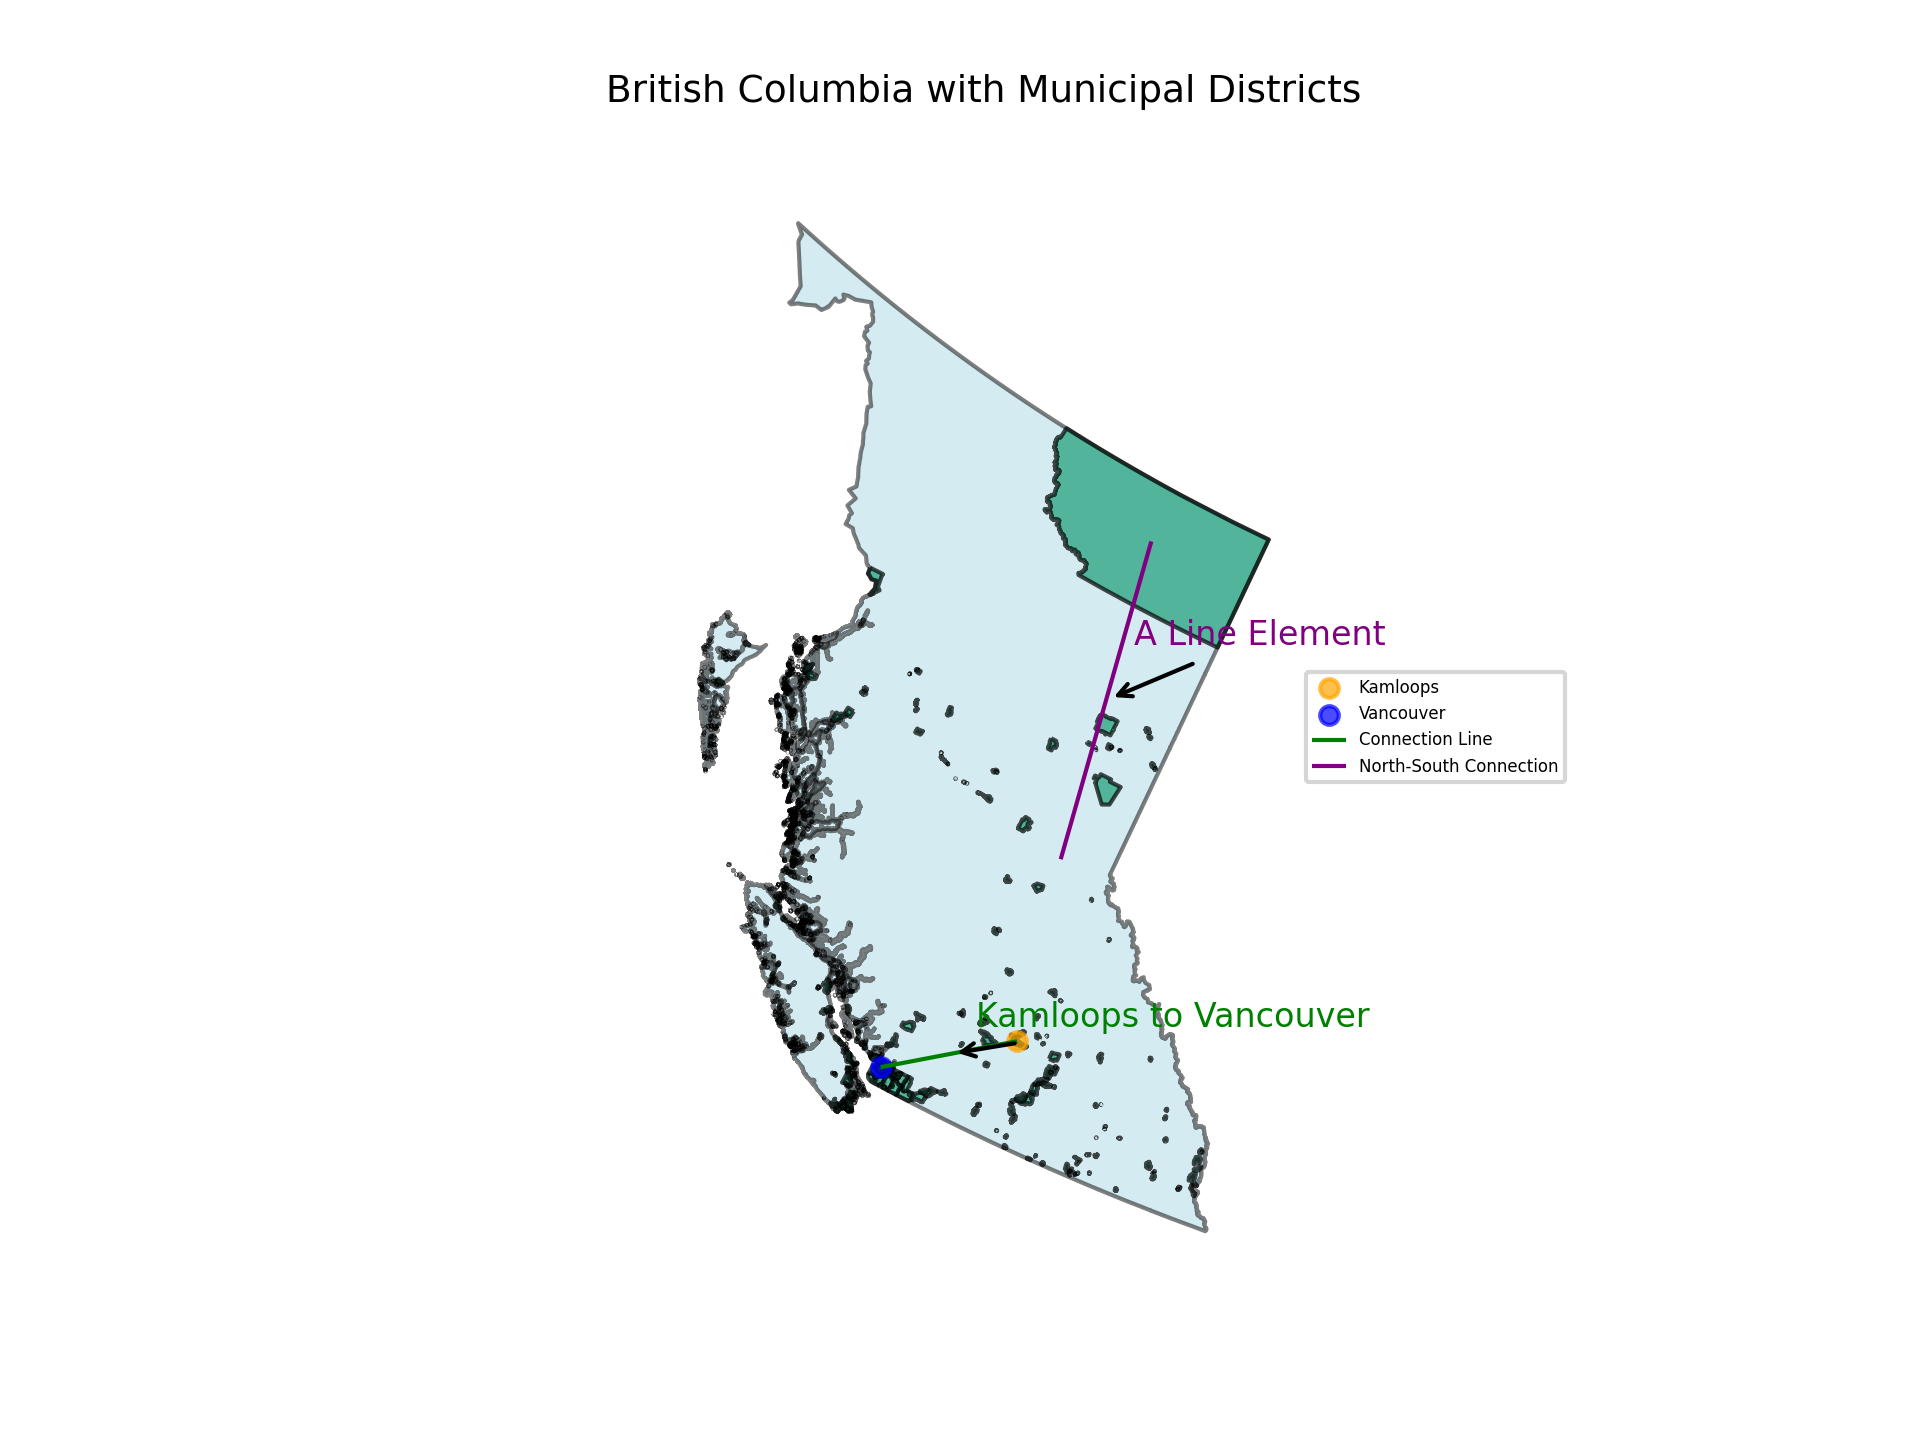
\includegraphics[width=0.9\textwidth]{../src_test/results/test_BC_map.png}
    \caption{\textit{Example of a map showing the location of Kamloops and Vancouver in BC. 4 points and two lines were added to the map.}}
    \label{fig:test_BC_map}
\end{figure}

Figure \ref{fig:test_BC_map} shows an example of a map showing the location of Kamloops and Vancouver in BC.
I downloaded the geographic data from government website, including: \href{https://open.canada.ca/data/en/dataset/a883eb14-0c0e-45c4-b8c4-b54c4a819edb/resource/12c03de6-c3f7-4f5f-bb5c-d479f2332842}{\textit{open.canada.ca}} and 
\href{https://catalogue.data.gov.bc.ca/dataset/municipalities-legally-defined-administrative-areas-of-bc/resource/0bd8e3d1-4d7f-4db8-a8b2-2cd4cd051074}{\textit{catalogue.data.gov.bc.ca}}. They provide the provincial and municipal boundaries of BC.

I managed to add basic geographic elements to the map, like points, lines and polygons and it worked well. If this part is considered worth to be included, 
i would spcifically try to create maps for Ontario Province with the Lake Huron-Lake Erie area and the Alberta Province with the fen complex distribution.

\subsection{Breakpoint quantile regression}

The detailed math part of breakpoint quantile regression is not discussed here, it could be left to work on later.
I tried to reproduce a similar result by using simulated data to validate the implementation with Python and my own code.

\paragraph{Continuous Breakpoint Regression:}
In continuous breakpoint regression, the relationship between the independent variable \(x\) and the dependent variable \(y\) is modeled such that the function remains continuous at the breakpoint \(c\). For example:

\[
y = 
\begin{cases} 
\beta_0 + \beta_1 x & \text{if } x \leq c \\
\beta_0 + \beta_1 c + \beta_2 (x - c) & \text{if } x > c
\end{cases}
\]

\paragraph{Discontinuous Breakpoint Regression:}
In discontinuous breakpoint regression, the relationship between \(x\) and \(y\) is allowed to have a jump at the breakpoint \(c\). For example:

\[
y = 
\begin{cases} 
\beta_0 + \beta_1 x & \text{if } x \leq c \\
\beta_2 + \beta_3 x & \text{if } x > c
\end{cases}
\]

\begin{figure}[!h]
    \centering
    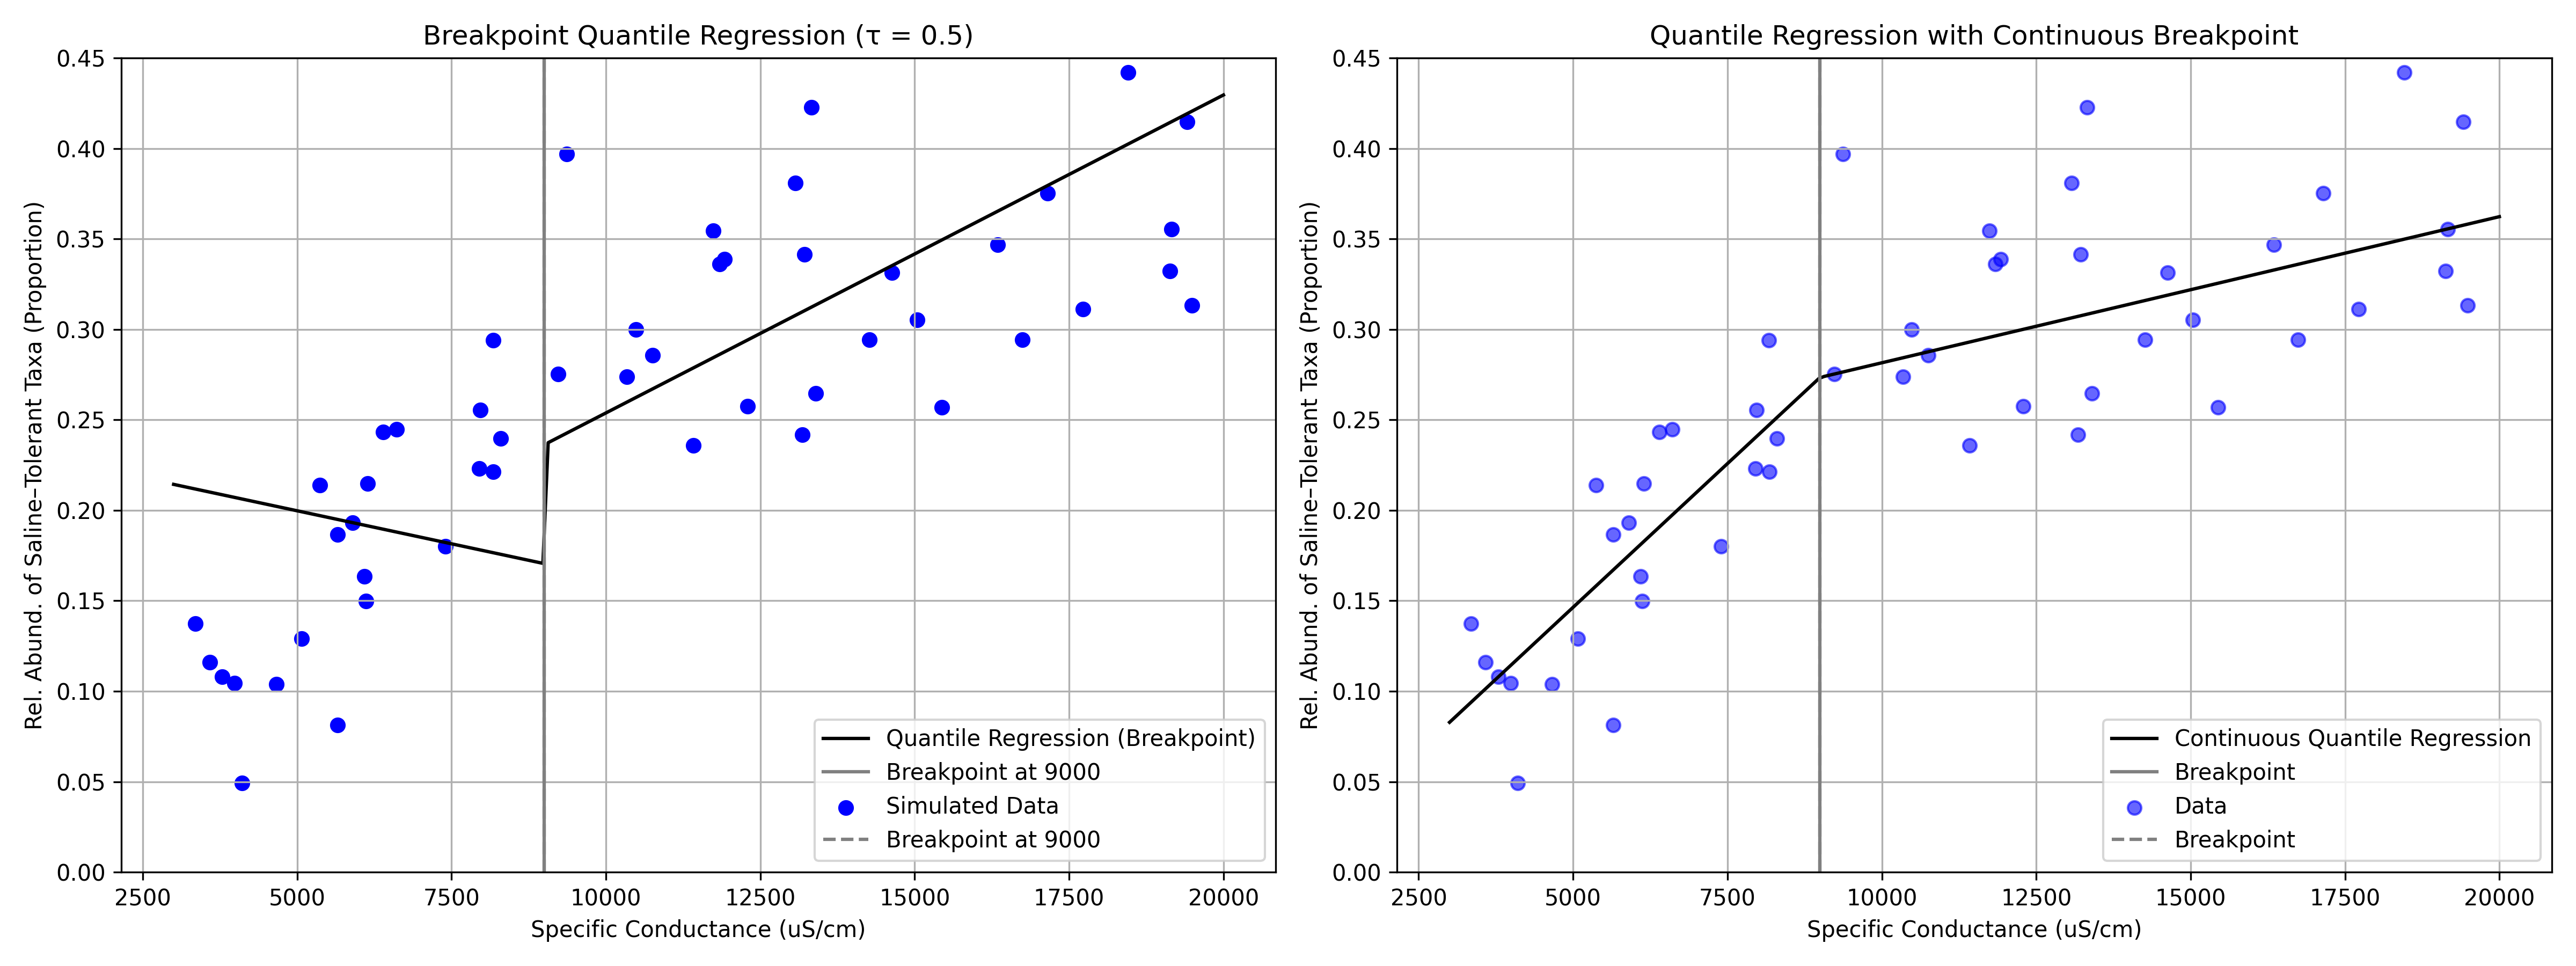
\includegraphics[width=0.9\textwidth]{../src_test/results/breakpoint_quantile_regression.png}
    \caption{\textit{Example of breakpoint quantile regression}}
    \label{fig:breakpoint_quantile_regression}
\end{figure}

It looks great, similar to one of the results by Vercruysse's work.

Later, i will try to incorporate this method with Bayesian formula and other methods to try to get a better result.


\subsection{PCA by Singular Value Decomposition (SVD)}

PCA is a method that was used in both Zhang's and Vercruysse 's work, i am also interested in this method.

These days i am reading the book \textit{Introduction to Linear Algebra, Fifth Edition(Gilbert Strang)} and very interested in the part
about singular value decomposition(SVD) and its importance in achieving PCA. Therefore, i tried to implement PCA using SVD by linear algebra 
with Python.

The SVD of \( X_c \) is given by:
\[
X_c = U \Sigma V^T
\]
where:
- \( U \) is an \( m \times m \) orthogonal matrix,
- \( \Sigma \) is an \( m \times n \) diagonal matrix with singular values on the diagonal,
- \( V \) is an \( n \times n \) orthogonal matrix.


The transformed data in the reduced space is given by:
\[
X_{\text{PCA}} = X_c V_k
\]
where \( V_k \) contains the top \( k \) principal components.

The reason of using SVD is that i want to try to adjust the PCA method and incoporate it with other methods 
to make it more flexible and specific for the data on hand.

\begin{figure}[!h]
    \centering
    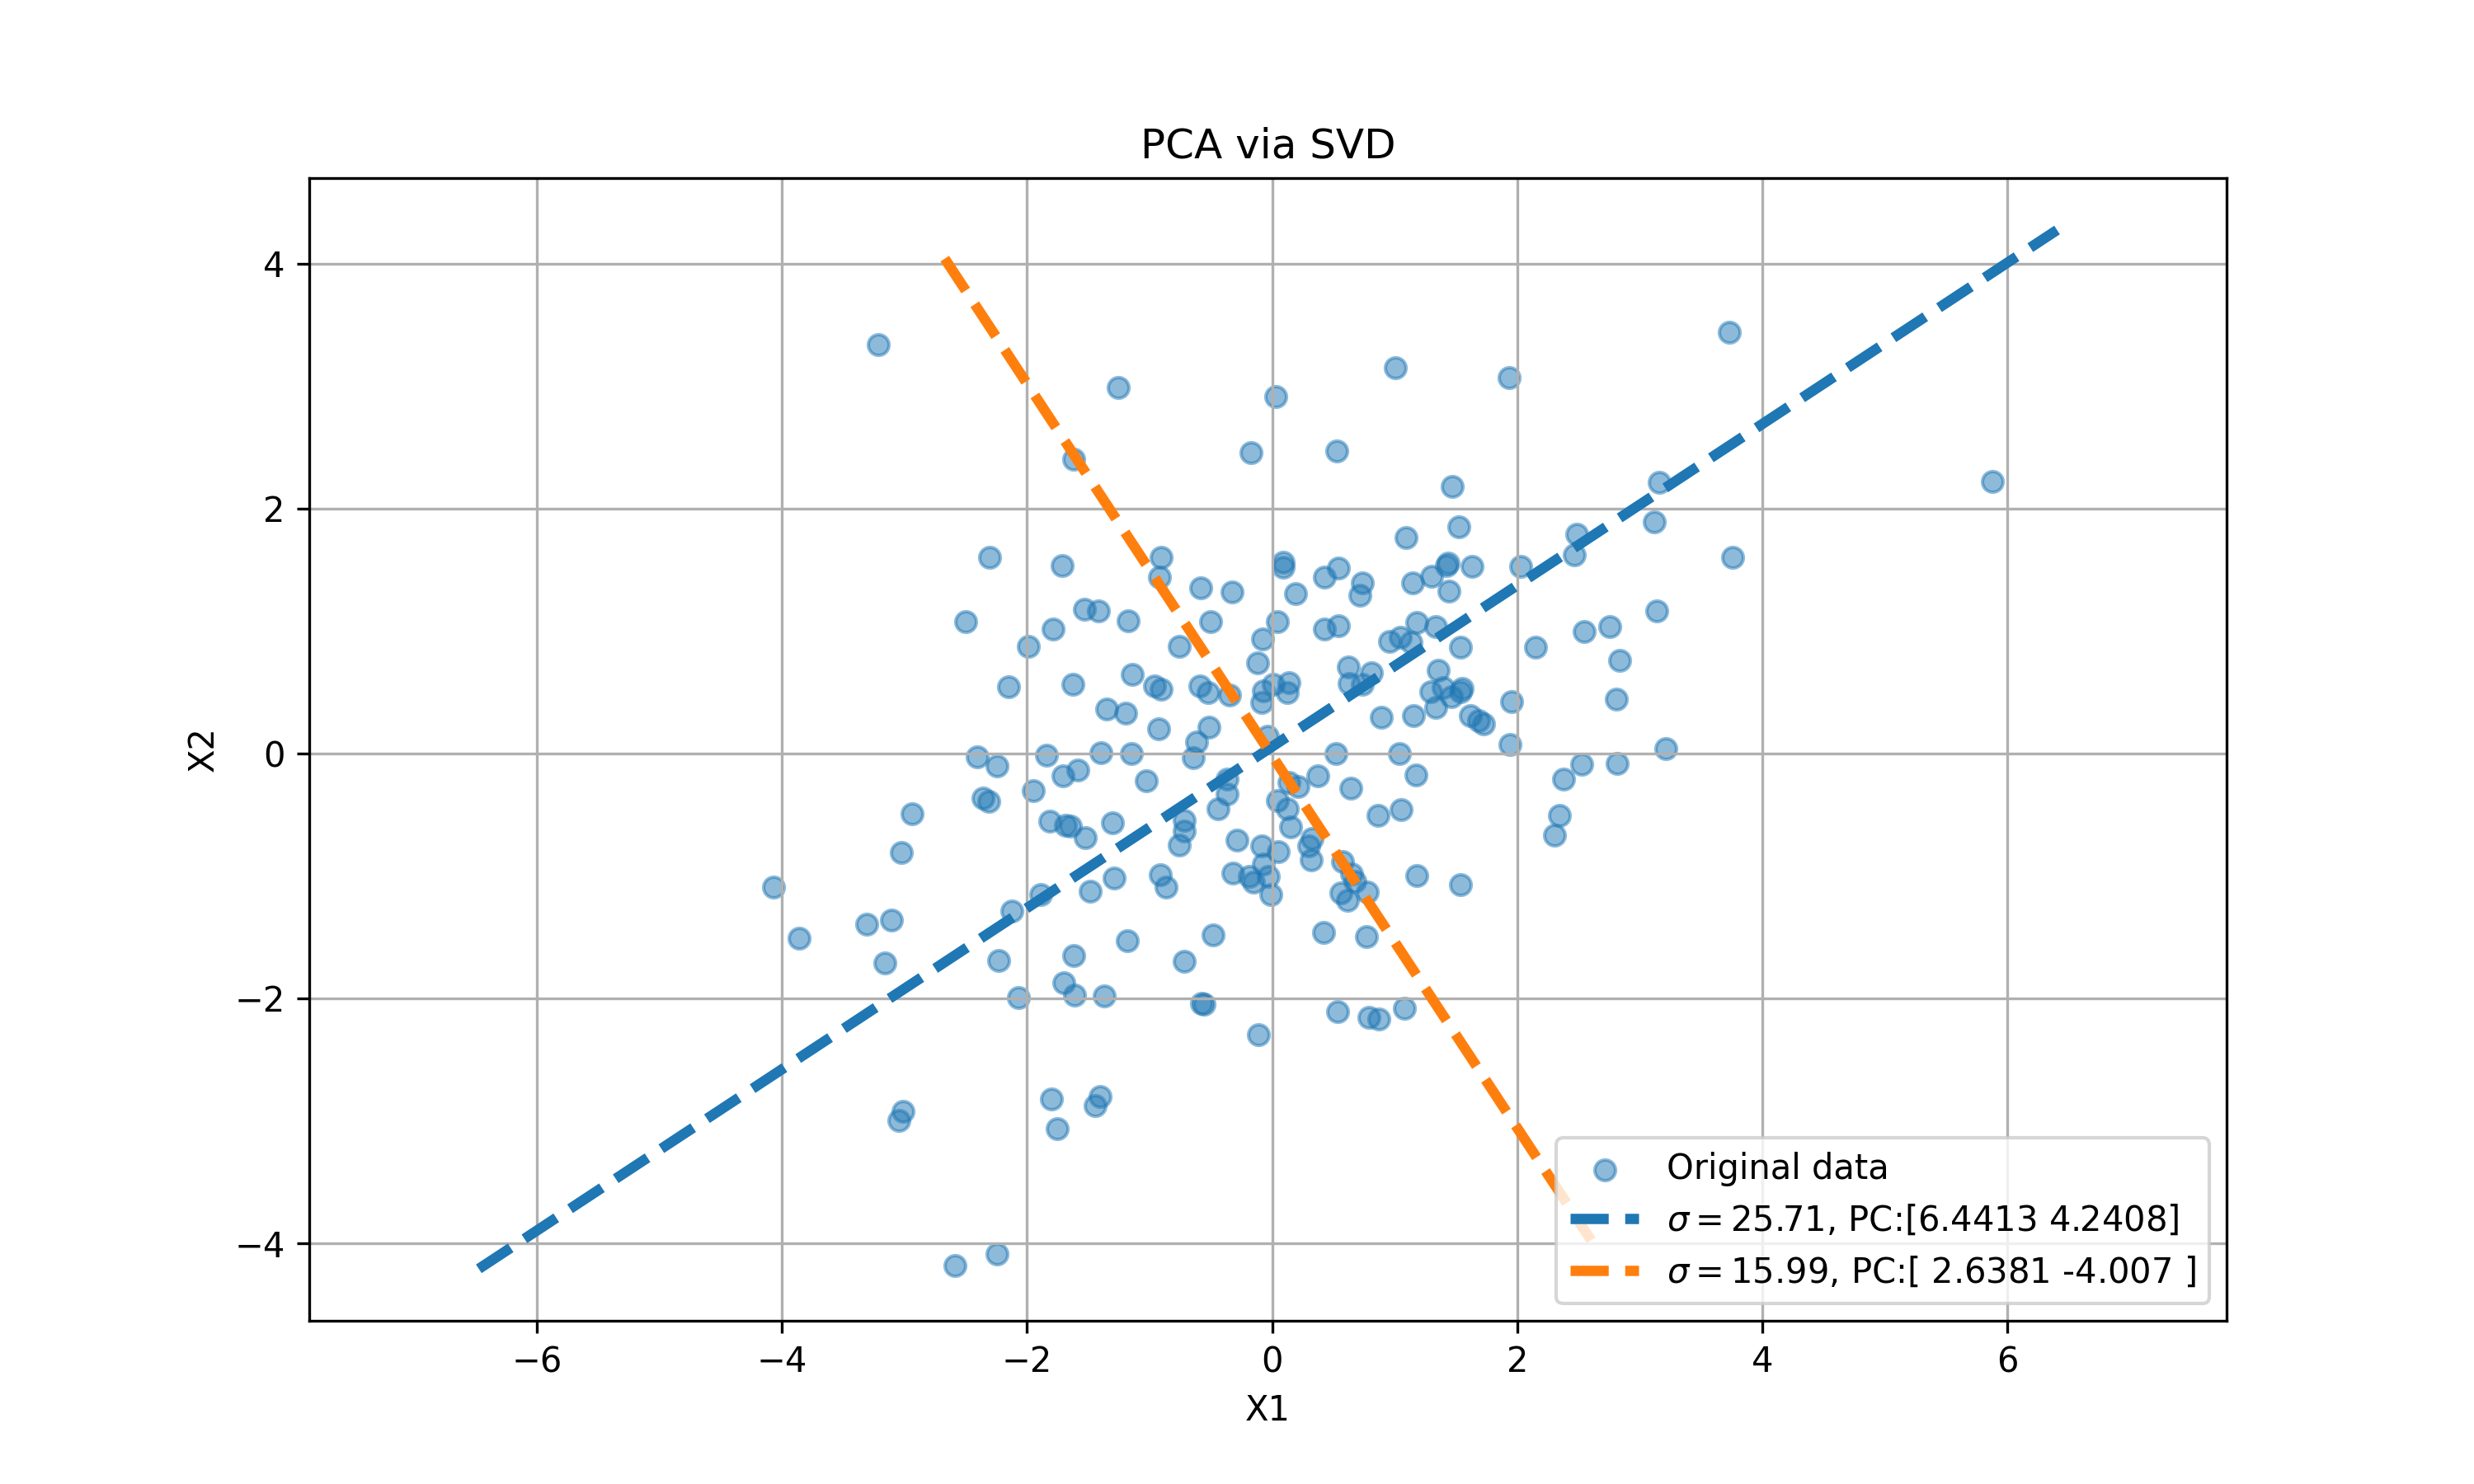
\includegraphics[width=0.9\textwidth]{../src_test/results/pca_svd.png}
    \caption{\textit{Example of PCA and SVD on the simulated data}}
    \label{fig:pca_svd}
\end{figure}

For example, figure \ref{fig:pca_svd} shows the PCA result by SVD, which is upon a simulated data.
One tentative idea could be to find a way to use less data(samples) to get relatively accurate 
singular values and vectors, which can be used to save time and effort in collecting data and computation.

\begin{figure}[!h]
    \centering
    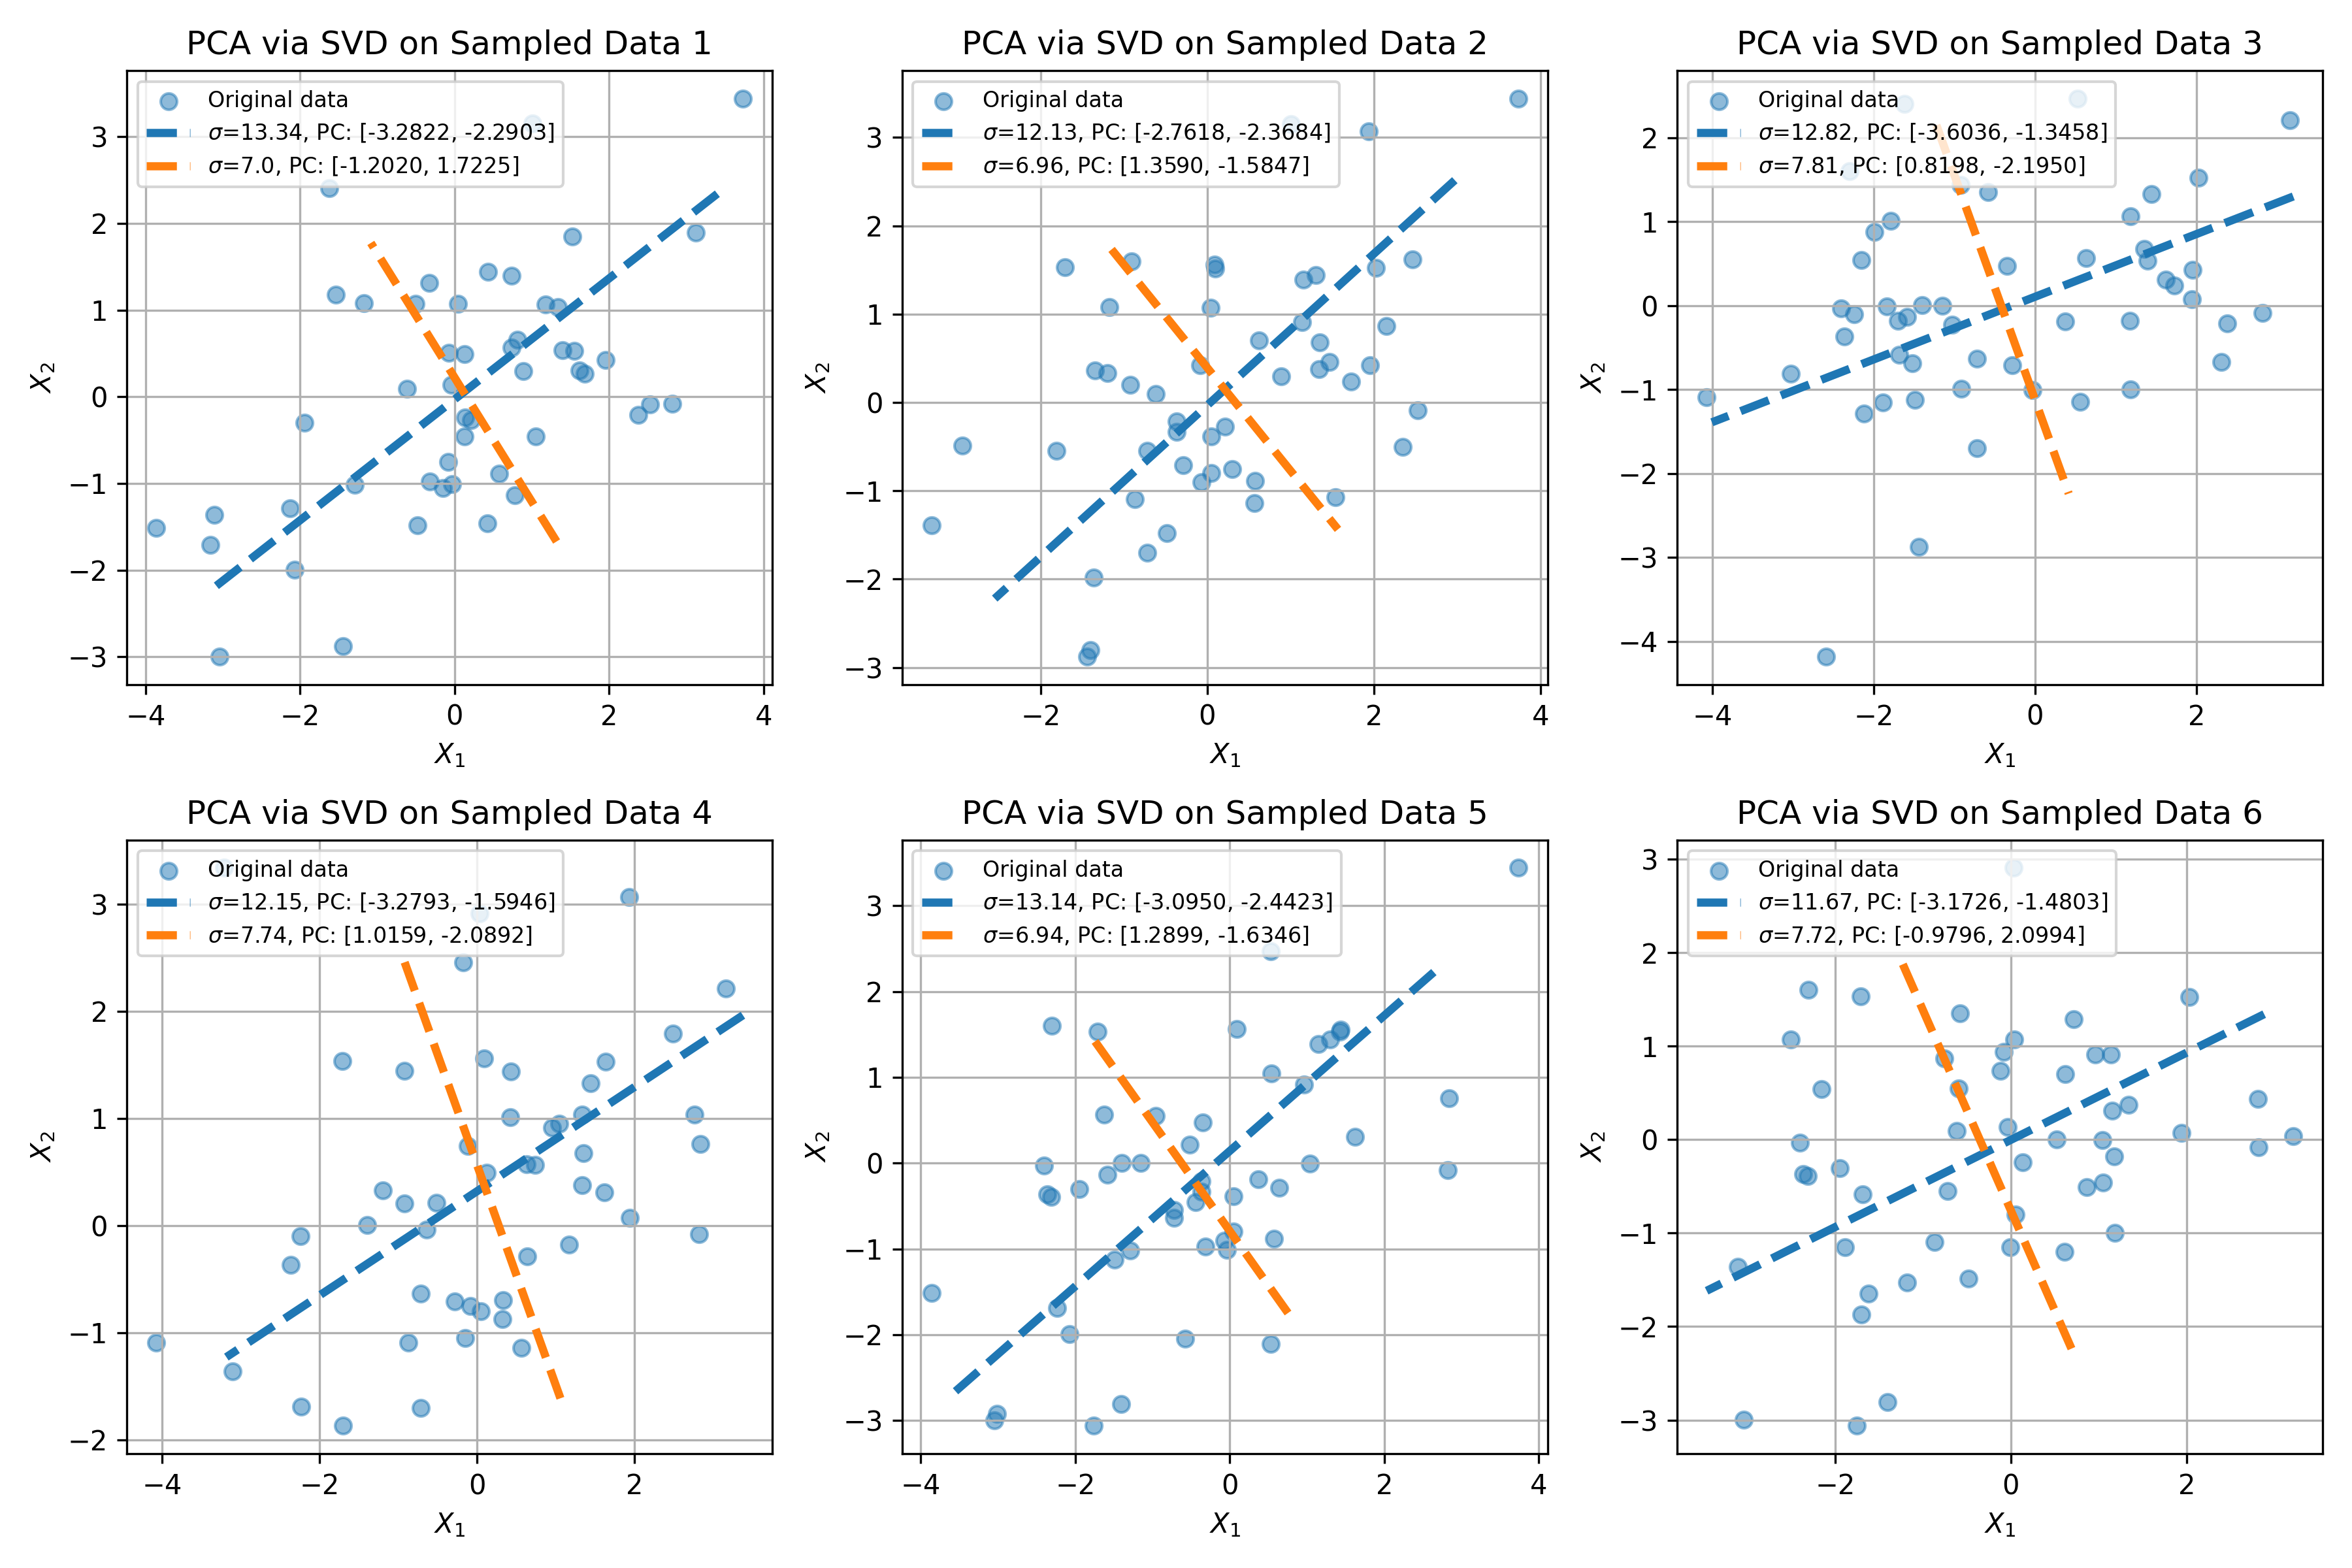
\includegraphics[width=0.9\textwidth]{../src_test/results/pca_svd_sampled_data.png}
    \caption{\textit{Example of PCA and SVD on sampled data from the simulated data}}
    \label{fig:pca_svd_2}
\end{figure}

Figure \ref{fig:pca_svd_2} shows the PCA result by SVD, which is upon different sampled sub-data from the 
original simulated data. The result is not as good as the one in figure \ref{fig:pca_svd}, which uses the whole data.
But this can be an aspect to explore along the work.


\end{document}